\begin{appendix}
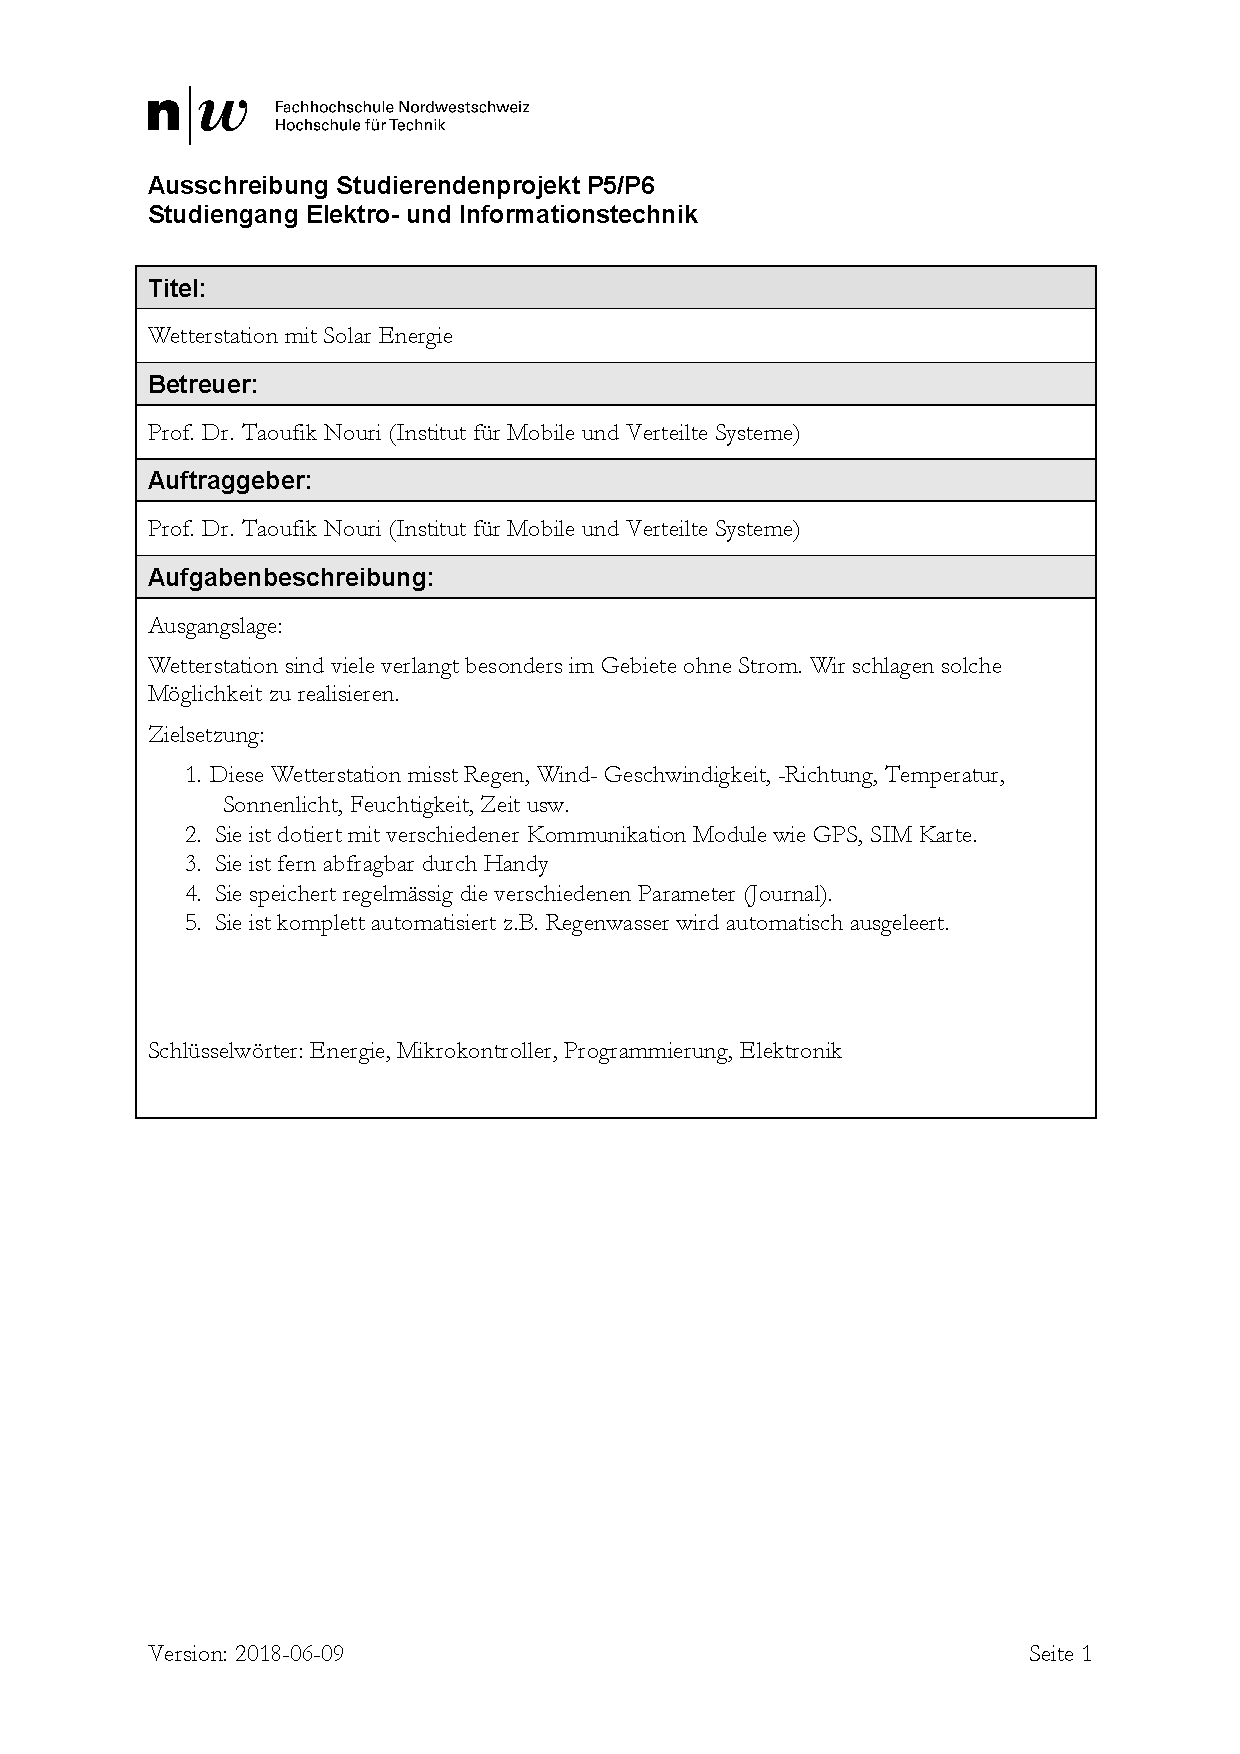
\includepdf[pages={1},nup=1x1,landscape=false,scale=0.85,offset=0 -40,pagecommand={\section{Lastenheft}\label{pdf:lastenheft}\thispagestyle{myheadings}}]{appendix/Auftragsbeschreibung.pdf} 
\newpage

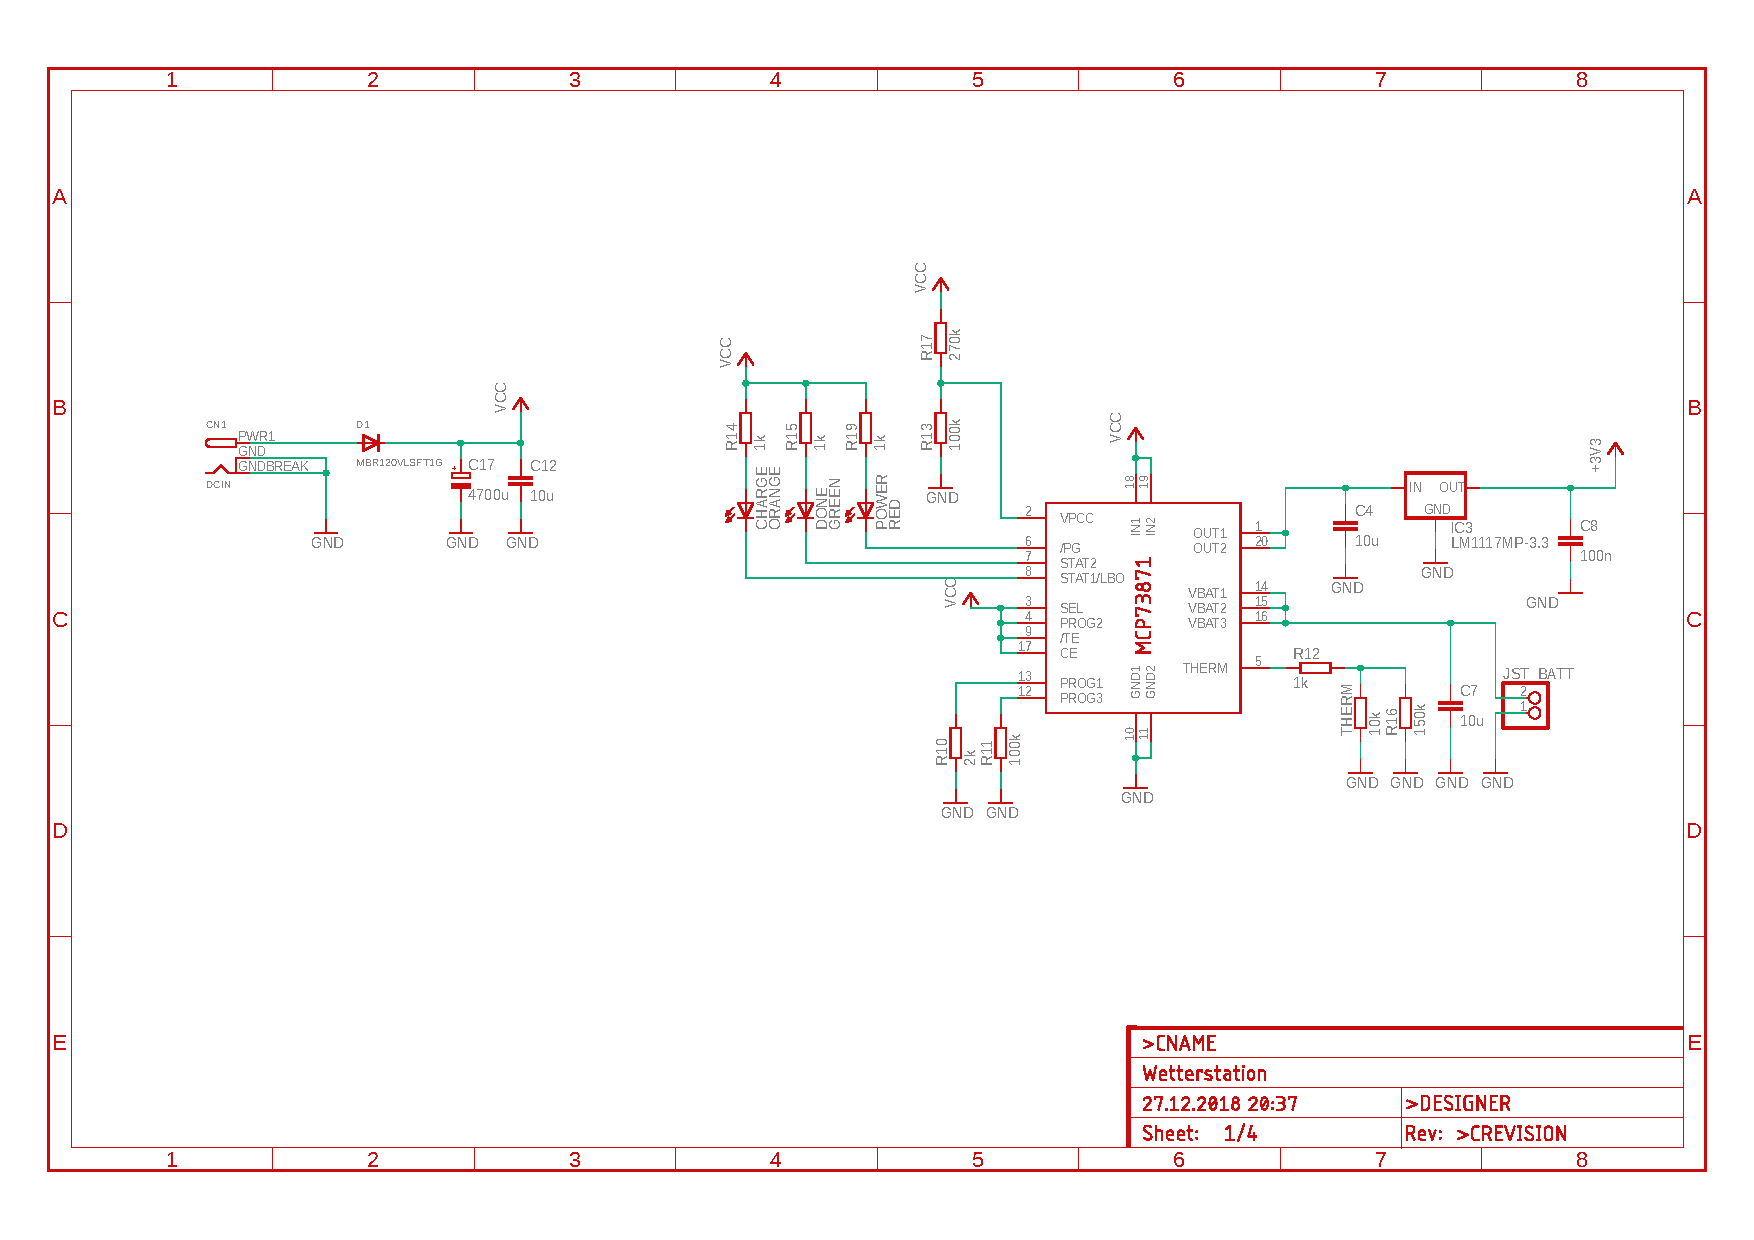
\includepdf[pages={1},nup=1x1,landscape=true,scale=0.75,offset=0 -40,pagecommand={\section{Schema}\label{pdf:schema} Hier wird das Schema der Wetterstation gezeigt, Dies ist ein Erstentwurf, welches anhand der Breakoutboards entworfen wurde und kann sich daher noch ändern.\thispagestyle{myheadings}}]{graphics/schema_und_layout/schematic.pdf} 

\includepdf[pages={2},nup=1x1,landscape=true,scale=0.85,offset=0 -40,pagecommand={\thispagestyle{myheadings}}]{graphics/schema_und_layout/schematic.pdf} 

\includepdf[pages={3},nup=1x1,landscape=true,scale=0.85,offset=0 -40,pagecommand={\thispagestyle{myheadings}}]{graphics/schema_und_layout/schematic.pdf}

\includepdf[pages={4},nup=1x1,landscape=true,scale=0.85,offset=0 -40,pagecommand={\thispagestyle{myheadings}}]{graphics/schema_und_layout/schematic.pdf}

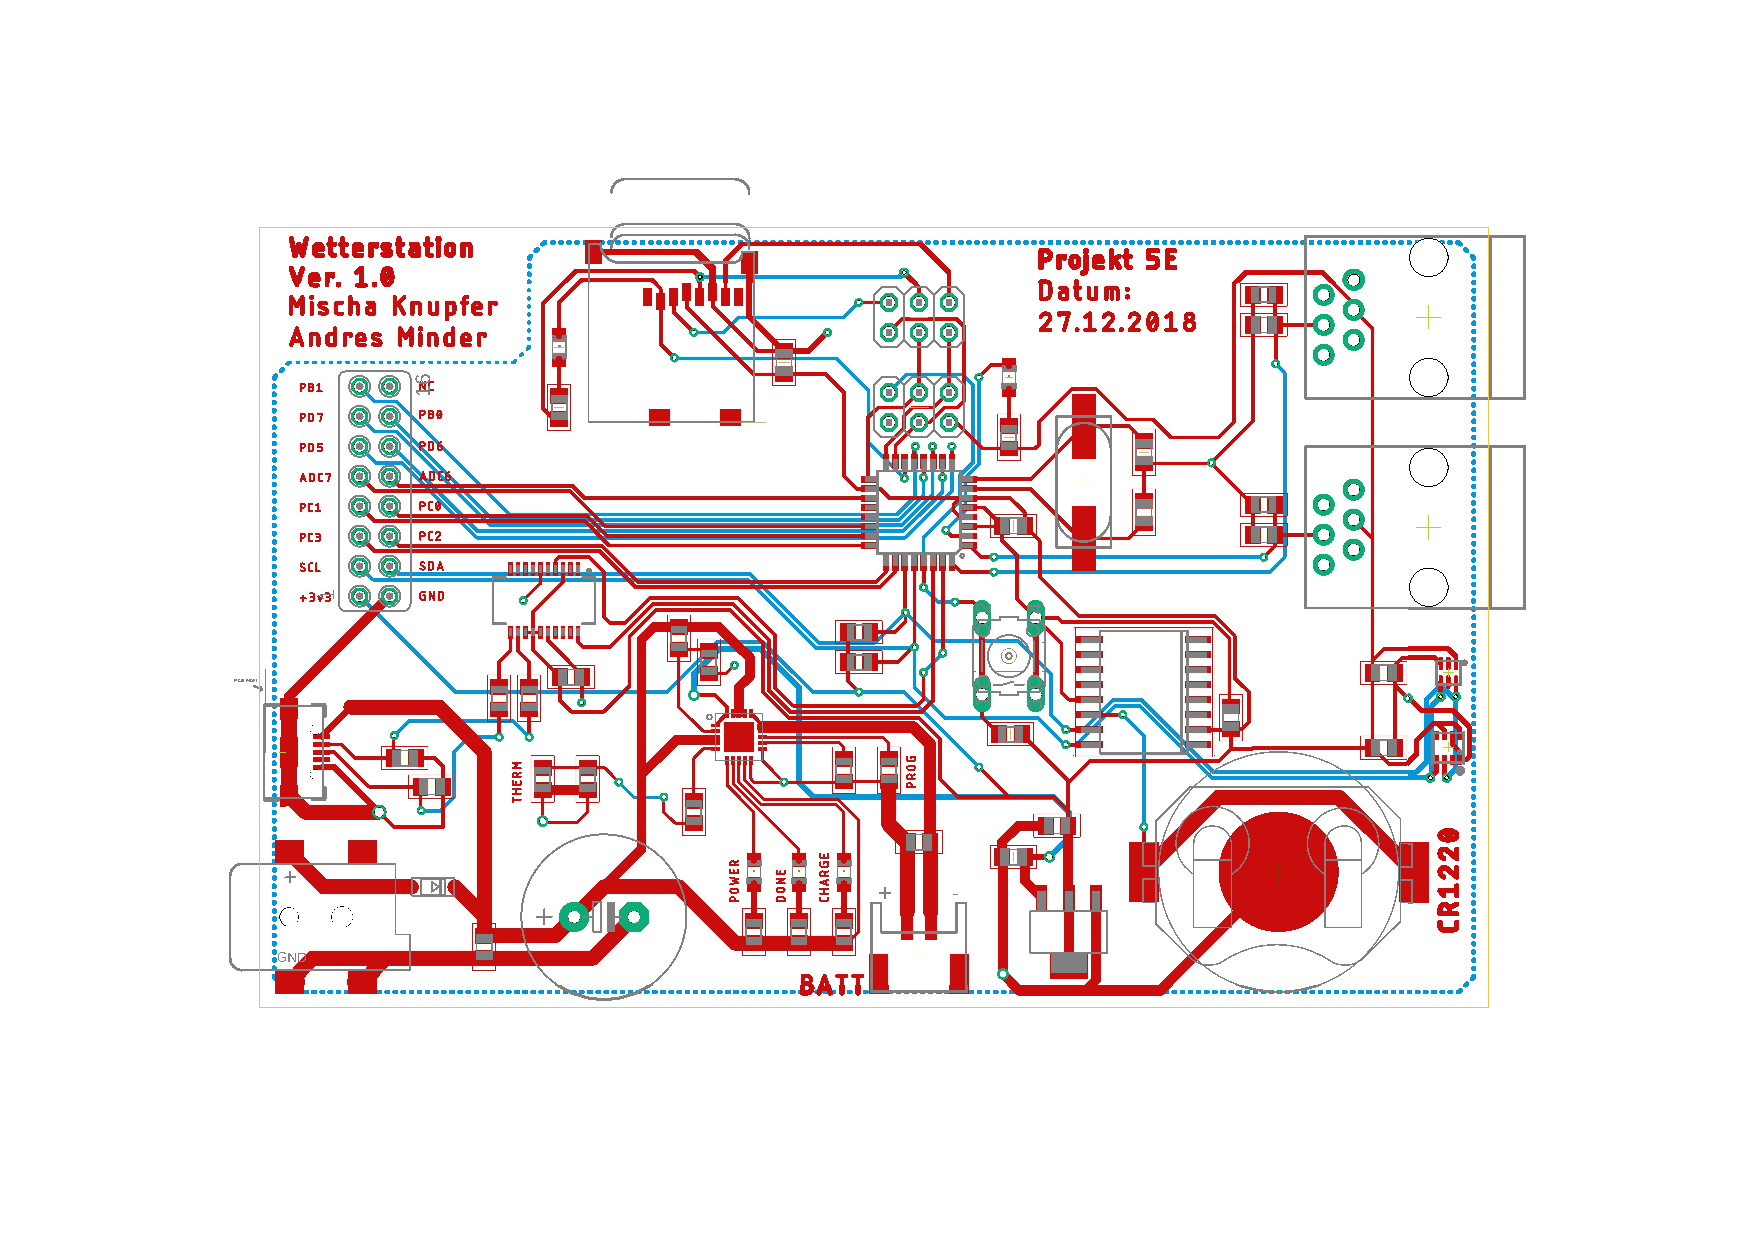
\includepdf[pages={1},nup=1x1,landscape=true,scale=0.85,offset=0 -40,pagecommand={\section{PCB-Design (Top View)}\label{pdf:pcb} Ein provisorisches PCB-Layout wurde designed, damit in einem weiterführenden Projekt Zeit eingespart werden kann. Im P5 wurde gemäss Aufgabenstellung jedoch auf ein Print verzichtet und nach Kapitel \ref{subsec:proto} vorgegangen.\thispagestyle{myheadings}}]{graphics/schema_und_layout/pcb_design.pdf}

\section{3D-Modellierung}
\label{pdf:3d_modellierung}
Die 3D-Modellierung zeigt ein 3D-Modell des erstellten provisorischen PCB-Layouts. Dieses PCB-Layout, und damit auch das anschauliche 3D-Modell, sind nur provisorisch und können sich noch ändern.
%{\begin{minipage}[b][\textheight][t]{0.49\textwidth}
%\centering
%\captionof{figure}{Top View}
%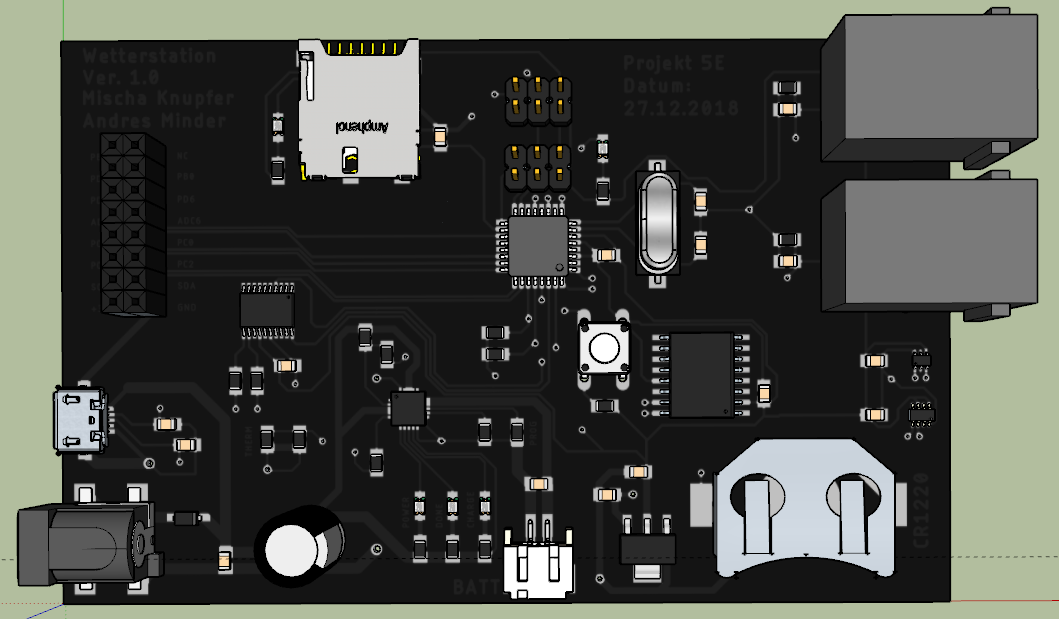
\includegraphics[width=\textwidth]{graphics/3D_Model/3d_topview.PNG}
%\label{fig:3d_topview}
%\end{minipage}}
%{\begin{minipage}[b][\textheight][t]{0.49\textwidth}
%\centering
%\captionof{figure}{Bottom View}
%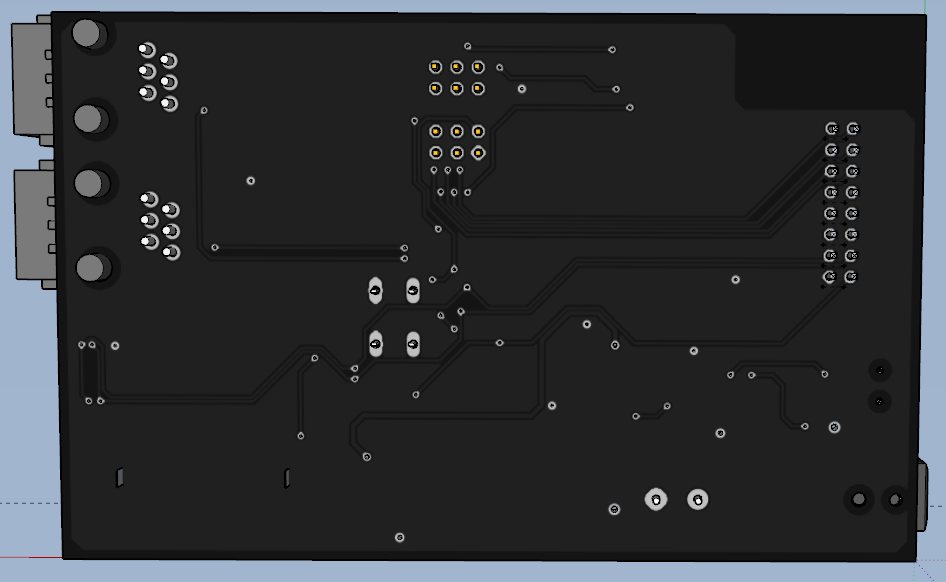
\includegraphics[width=\textwidth]{graphics/3D_Model/3d_groundview.PNG}
%\label{fig:3d_bottomview}
%\end{minipage}}

\begin{figure}[hbtp]
\centering
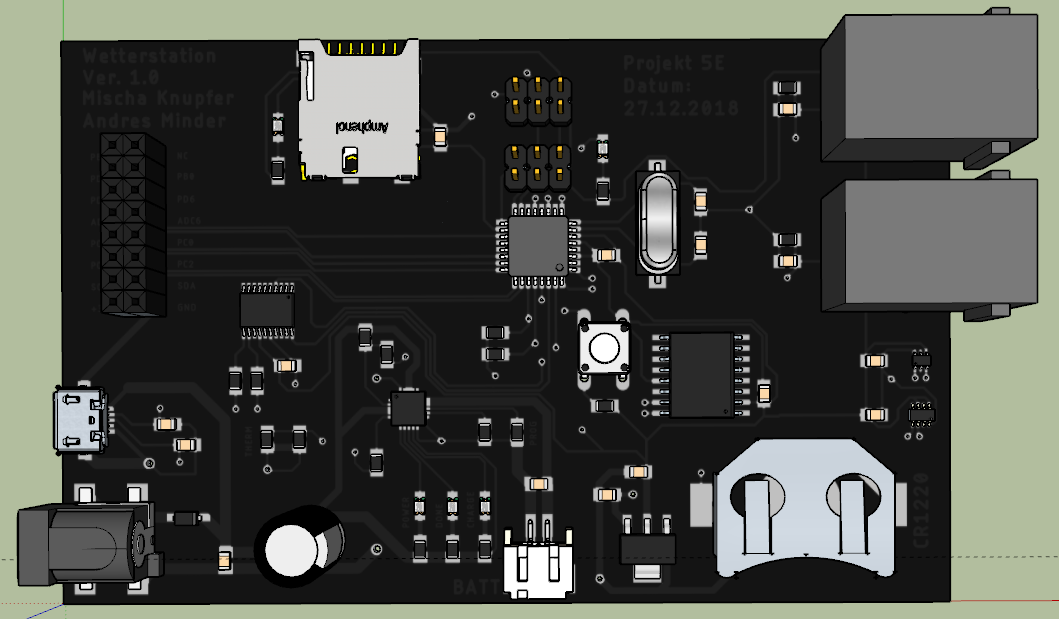
\includegraphics[width=0.5\textwidth]{graphics/3D_Model/3d_topview.PNG}
\caption{Top View}
\label{fig:3d_topview}
\end{figure}

\begin{figure}[hbtp]
\centering
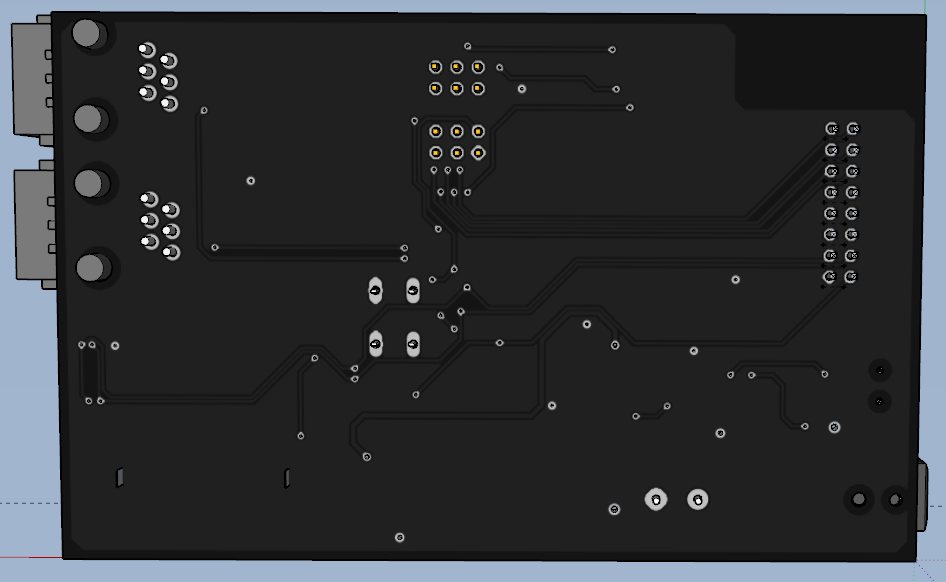
\includegraphics[width=0.5\textwidth]{graphics/3D_Model/3d_groundview.PNG}
\caption{Bottom View}
\label{fig:3d_bottomview}
\end{figure}

\begin{figure}[hbtp]
\centering
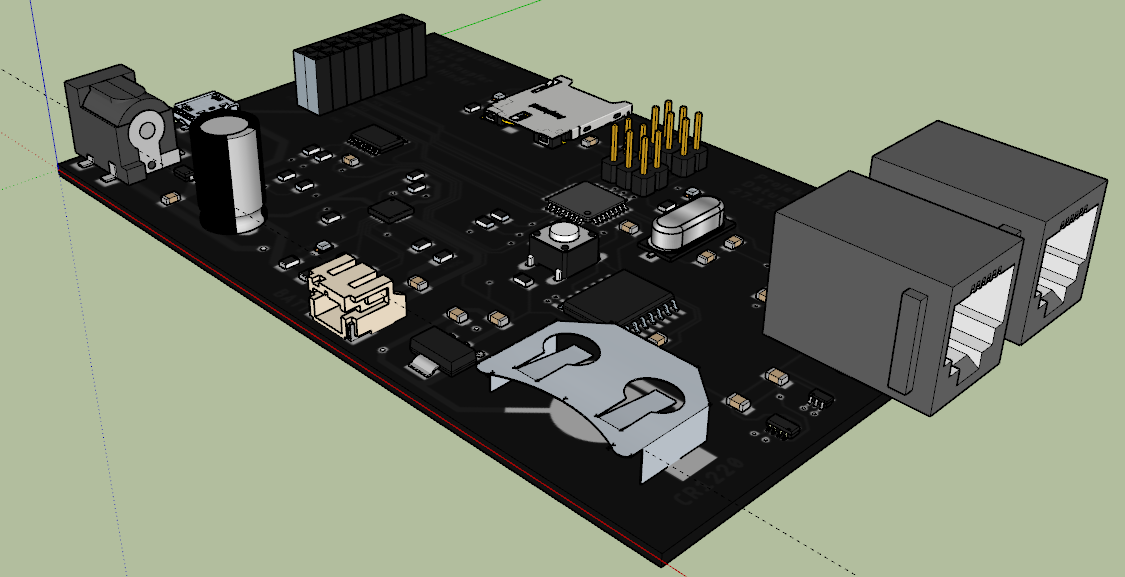
\includegraphics[width=0.5\textwidth]{graphics/3D_Model/3d_dioganalFrontRight_view.PNG}
\caption{Side View}
\label{fig:3d_sideview}
\end{figure}


\end{appendix}

